%% ID: firing_a_canon
%% TITLE: Firing a Canon
%% TYPE: question
%% QUESTIONTYPE: symbolic
%% CONCEPTS: energy, momentum, impulse, eq_of_motion_diff
%% VIDEOS: 
%% LEVEL: 3
%% TOPIC: mechanics/dynamics
%% ORDER: 9

\begin{problem}[A1972AMIIQ2l] %Nice impulse/work/SUVAT question with multiple methods of solving. Requires some frames of reference initially - a bit tricky.
{\begin{enumerate}
	\item A gun of mass \value{M}{1000}{kg} stands on horizontal ground and can move horizontally against a recoil mechanism. With its barrel raised at an angle of \value{\theta}{60^{\circ}}{} to the ground, it fires a projectile of mass \value{m}{20}{kg} with a speed \value{u}{306}{m\,s^{-1}} \stress{relative to the barrel}. Calculate the horizontal impulse on the gun and the total kinetic energy produced by the explosion which fired the projectile. Clearly state the units in which both quantities are measured.
	\item If the recoil mechanism brings the gun to rest when it has moved back \value{r}{25}{cm}; find the force exerted by the mechanism, assuming it to be constant.
	\item Show that the time taken for the gun to recoil through this distance is $\frac{1}{6}${s}.
\end{enumerate}
}
{\stress{Used with permission from UCLES, A Level Applied Mathematics, June~1972, Paper~2, Question~2.}}
{\begin{enumerate}
	\item The first key thing to realise is that the speed of the projectile is given relative to the barrel, not the ground (since the same impulse acts on two things at rest, the ground frame is the zero momentum frame [ZMF]). Resolving the speed to the horizontal, \vari{u \cos(\theta)}, and then drawing a diagram of the gun and projectile as particles will aid in finding the horizontal speeds in the ZMF, as in Figure \ref{fig:Dynamics_gun_speeds}. The barrel is moving away from the projectile, and so the speed of the projectile will be less than \vari{u \cos(\theta)} by some amount \vari{v}, the speed of the gun recoiling.

\begin{figure}[h]
\centering
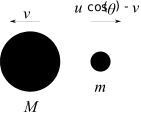
\includegraphics[width=0.2\textwidth]{../../../figures/Dynamics_gun_speeds.eps}
\caption{}
\label{fig:Dynamics_gun_speeds}
\end{figure}

Since momentum is conserved, their momenta must be equal:
\begin{align*} 
(M)(v) &= (m)(u \cos (\theta) - v) \\  
\frac{M}{m} &= \left( \frac{u \cos(\theta)}{v} - 1 \right) \\  
\frac{M}{m} + 1 &= \frac{u \cos(\theta)}{v} \\ 
v &= \frac{u \cos(\theta)}{\frac{M}{m} + 1} \\ 
v &= \frac{(306)(\frac{1}{2})}{\frac{(1000)}{(20)} + 1} \text{ ms}^{-1} = 3 \text{ ms}^{-1}
 \end{align*}

The impulse is the change in momentum, and so the momentum of either body will give the horizontal impulse: \vari{I} = \vari{Mv} = \quantity{(1000)(3)}{} = \vari{m(u \cos(\theta) - v)} = \value{(20)(153 - 3)}{3000}{kg\,m\,s\sup{-1}}.
The kinetic energy produced by the explosion is then the sum of the two kinetic energies: $E = \frac{1}{2}Mv^{2} + \frac{1}{2}m\left[\frac{(u \cos(\theta) - v)}{\cos(\theta)}\right]^{2} = \frac{1}{2}(1000)(3)^{2} + \frac{1}{2}(20)(306 - 6)^{2} =$ \quantity{904500}{ J} where we have been careful to get the full speed of the projectile relative to the ground.

Impulse is measured in \quantity{}{kg\,m\,s\sup{-1}} (kilogram metres per second) or \quantity{}{N\,s} (Newton seconds), where the former is expressed in SI base units but the two are completely equivalent (this can be shown by substituting in the definition \quantity{1}{N} $\equiv$ \quantity{1}{kg\,m\,s\sup{2}}). Energy is measured in \quantity{}{J} (Joules) or \quantity{}{kg\,m\sup{2}\,s\sup{-2}} (kilogram meters squared per second squared), again equivalent units.
	\item If the force is constant, then the acceleration is constant and so we can use Newton's Second Law and the SUVAT equation \value{v^{2}}{u^{2} + 2as}{}. Since right is our positive direction, we have \value{s}{-r}{,} \value{u}{\frac{-I}{M}}{} and \value{v}{0}{m\,s\sup{-1}} so:
\begin{align*} 
a &= \frac{v^{2} - u^{2}}{2s} = \frac{-\left( \frac{-I}{M} \right)^{2}}{-2r} = \frac{I^{2}}{2M^{2}r} \\ 
&= \frac{(3000)^{2}}{2(1000)^{2}(0.25)} \text{ ms}^{-2} = 18 \text{ ms}^{-2} 
\end{align*}
and then \value{F}{ma}{} gives the force acting on the gun:
\begin{align*} 
F &= M \left( \frac{I^{2}}{2M^{2}r} \right) = \frac{I^{2}}{2Mr} \\ 
&= \frac{(3000)^{2}}{2(1000)(0.25)} \text{ N} = 18000 \text{ N} 
\end{align*}
There is another way of obtaining this answer, using energy. The only way to dissipate the kinetic energy of the gun, to bring it to a stop, is work against the resistive force from the recoil mechanism. Thus the work done by the recoil mechanism stopping the gun, the force times the distance \vari{r}, must equal the gun's initial kinetic energy: \vari{W} = \value{Fr}{\frac{1}{2}Mv^{2}}{} and so:
\begin{equation*} 
F = \frac{\frac{1}{2}Mv^{2}}{r} = \frac{(1000)(3)^{2}}{2(0.25)} = \mbox{\quantity{18000}{N}} 
\end{equation*} as before.

	\item Again we can use a SUVAT equation to find the time taken, \value{s}{\left( \frac{u + v}{2} \right)t}{} with \vari{s}, \vari{u} and \vari{v} as before:
\begin{align*} 
t &= s \left( \frac{2}{u + v} \right) = (-r) \left( \frac{2}{\left( -\frac{I}{M} \right)} \right) = \frac{2Mr}{I} \\ 
&= \frac{(2)(1000)(0.25)}{3000} \text{ seconds} = \frac{1}{6} \text{ s} 
\end{align*} as required.

Another way of solving this would be to realise that the change in momentum of the gun from recoiling to stationary is equal to the impulse from the recoil mechanism: \vari{\Delta p} = \value{I_{rm}}{Ft}{} or:
\begin{equation*} 
t = \frac{\Delta p}{F} = \frac{(1000)(3)}{(18000)} \text{ s} = \frac{1}{6} \text{ s}
 \end{equation*}

\end{enumerate}}
\end{problem}